Il modello M/G/1 simboleggia un sistema che ha un solo servitore, in cui gli arrivi sono markoviani (o senza memoria), mentre il servizio segue una distribuzione generica $F_y(a)$. Per fissare le idee, diciamo che il tasso degli arrivi \`e pari a $\lambda$, mentre il tasso di servizio \`e pari a $\mu$.
La markovianità degli arrivi \`e giustificata dal fatto che in una rete grande, le possibili sorgenti di transazione sono molte e indipendenti; mentre la stazionarietà/omogeneità \`e giustificata dal fatto che il comportamento della rete \`e tempo invariante. La statistica dei tempi di inter-arrivo \`e esponenziale perch\`e \`e conseguenza della poissonianità e omogeneità.
Il fatto che il sistema abbia un solo servitore, non significa che anche il numero di minatori dell'intera rete sia uno, ma significa che la stessa transazione (che \`e il cliente del sistema) viene servita da tutti gli $m$ minatori. Dunque, in termini di teoria delle code, \`e come avere un sistema formato da una sola coda in cui il cliente viene servito da un'unica entità composta da $m$ minatori che la servono contemporaneamente.
Il modello M/G/1 \`e utilizzato in letteratura per il calcolo dei tempi di conferma delle transazioni e dei ritardi e dello studio dei fattori che li influenzano, come ad esempio la dimensione del blocco o il numero di transazioni.

%*****************************************************************
\section{Rappresentazione come catena di Markov}
Il modello M/G/1 si può analizzare facilmente se lo si rappresenta come una catena di Markov. Per farlo, però, bisogna dimostrare la prorpietà di Markov e trovare lo stato e la sua statistica. Fatto questo, poi, si possono ricavare le statistiche e i momenti di tutte le metriche. Si inizia considerando il numero totale di clienti $x(t)$ nel sistema negli istanti immediatamente successivi alla $n$-esima partenza dal sistema, denominati $t_n^+$%
.\footnote{Il termine \textit{clienti} \`e usato per questo modello in maniera generale. Infatti, ci si può riferire ai clienti sia come transazioni sia come blocchi.} Indicando con $x_n:= x(t_n^+)$ il numero di clienti nel sistema immediatamente dopo il verificarsi della $n$-esima partenza, possiamo scrivere le seguenti relazioni che ne specificano la dinamica~\cite{libro:tele}:
\begin{itemize}
\item se la partenza $n$-esima lascia il sistema vuoto, prima che si verifichi una nuova partenza, \`e necessario attendere l’arrivo di un cliente e la fine del suo tempo di servizio. Supponiamo che in questo lasso di tempo, arrivi un numero di clienti pari alla variabile aleatoria $v_n$. Dunque, un instante dopo la partenza $n$-esima, il numero totale di clienti diventa pari a $v_n$. In formula: \begin{equation} x_{n+1}=v_n \end{equation}
\item se dopo la partenza $n$-esima il sistema non \`e vuoto, il prossimo cliente in coda accede al servizio e si aggiungono poi $v_n$ clienti al sistema. Dunque, dopo la partenza, avremo $x_n-1$ clienti rimanenti e in più i $v_n$ appena arrivati. In formula: \begin{equation} x_{n+1}=x_n-1+v_n \end{equation}
Possiamo unificare le due equazioni precedenti utilizzando la funzione indicatrice:
\begin{equation}\label{eq:chi}\chi \{x_n>0\}=\begin{cases} 1 & \text{se}\quad x_n>0\\ 0 & \text{se}\quad x_n=0 \end{cases}\end{equation}
ottenendo dunque:
\begin{equation}\label{eq:stato} x_{n+1}=x_n+v_n-\chi \{x_n>0\}. \end{equation}
\end{itemize}
Ora, per poter dire che il sistema M/G/1 evolve secondo una catena di Markov, bisogna dimostrare che la descrizione statistica fatta per gli istanti $t_n^+$, valga \textit{per ogni} istante di osservazione. 
Un modo per dimostrarlo \`e il seguente. Si può notare che, asintoticamente, il numero $x_n$ di clienti nel sistema subito dopo una partenza, \`e distribuito come $x(\tau_m^-)$, che \`e il numero di clienti nel sistema appena prima l'arrivo di un nuovo cliente. Dopodich\`e, si può sfruttare la proprietà PASTA, che dice che gli arrivi poissoniani ``vedono" davanti a loro, la distribuzione asintotica dello stato $x(t)$. Dunque, $x(\tau_m^-)$ \`e distribuita come $x(t)$ per $t \to \infty$. Ma allora, se asintoticamente $x_n$ \`e distribuita come $x(\tau_m^-)$ che, a sua volta, \`e distribuita come $x(t)$, vale che per $n \to \infty$, $x_n$ converge alla distribuzione di $x(t)$. In conclusione, in regime stazionario e in qualsiasi istante di osservazione, si ha un'unica descrizione statistica dello stato~\cite{libro:tele}.

%*****************************************************************
\section{Calcolo del tempo medio di attesa in coda}
Ora, si vuole riportare il calcolo del tempo medio di attesa in coda $E[T_Q]$, che in ambito criptovalute, viene visto come il \textit{ritardo} del tempo di conferma di una transazione. Per tutti gli altri momenti delle metriche, si consiglia di vedere~\cite[586-587]{libro:tele}.
Viene sfruttata la tecnica \textit{tagged-job}, nella quale si ``tagga" un arrivo arbitrario e si ragiona sul tempo speso in coda proprio da questo arrivo selezionato~\cite{libro:tempo-MG1}. Si ipotizza che tutte le variabili in gioco siano i.i.d.
Verrà utilizzata la seguente notazione:
\begin{itemize}
\item $\rho=\frac{\lambda}{\mu}=$ fattore di carico;
\item $T_Q=$ tempo in coda;
\item $N_Q=$ numero clienti in coda;
\item $N_Q^A=$ numero clienti in coda visti dal cliente ``taggato";
\item $S=$ tempo di servizio $\implies$ $E[S]=\frac{1}{\mu}$;
\item $S_i=$ tempo di servizio $i$-esimo cliente;
\item $S_e=$ tempo di servizio visto dal cliente ``taggato".
\end{itemize}
Allora:
\begin{subequations}\begin{align}E[T_Q] & \notag =E[\text{tempo di servizio dei clienti in coda prima del ``tag"}]\\ \notag & +E[\text{tempo di servizio residuo del cliente in servizio}]= \\ \notag
&=E[\sum_{i=1}^{N_Q^A} S_i]+E[\text{tempo di servizio residuo del cliente in servizio}]=\\ \notag
&\underset{\text{indip.}}{=} E[N_Q^A] E[S] + P[\text{unico servitore \`e impegnato}] E[S_e]=\\ 
&\label{eq:tempo-coda} \underset{\text{PASTA}}{=} E[N_Q] E[S] + \rho E[S_e]=\\ \notag
&\underset{\text{Little}}{=} E[T_Q] \lambda E[S] + \rho E[S_e]=\\ \notag
&=\rho E[T_Q] + \rho E[S_e]=\\ 
&= \frac{\rho}{1-\rho} E[S_e]. \end{align}\end{subequations}

%*****************************************************************
\section{Analisi della statistica del ritardo}
Nell'articolo~\cite{art2:MG1}, si parla dei fattori che impattano i ritardi delle transazioni Bitcoin sfruttando la teoria delle code. Per \textit{ritardo} si intende quell'intervallo temporale che la transazione deve attendere prima di essere scelta per far parte di un blocco. Utilizzando la nomenclatura della teoria delle code e considerando le transazioni come clienti, il ritardo equivale al tempo medio di attesa in coda, che in questo caso viene chiamata in gergo \textit{mining pool}. In~\cite[sez. 4]{art2:MG1} sono scritti i parametri considerati. Vengono riportati quelli più rilevanti:
\begin{itemize}
\item $\lambda$ \`e il tasso di arrivo di un gruppo di transazioni;
\item $\lambda_B$ \`e il tasso con cui vengono minati i blocchi (misurato in $blocchi/s$);
\item ogni blocco contiene in media $\tau$ transazioni;
\item $\lambda=\lambda_B \tau$ \`e il tasso di servizio delle transazioni;
\item $B$ \`e il tempo che intercorre tra la conferma di due blocchi (tempo inter-blocco). Inoltre vale che $E[B]=\frac{1}{\lambda_B}$;
\item $D$ \`e il ritardo di una transazione. In particolare, $D_{i,j}$ indica il tempo dall’ istante della conferma della $j$-esima transazione nel blocco $i$ fino all’istante di conferma dell'intero blocco.
\end{itemize}
Dopodich\`e, sfruttando la tecnica \textit{tagged-job}, gli autori hanno affermato che:
\begin{equation}\label{eq:ritardo} E[D]=\alpha E[B] + E[B_r], \end{equation} 
dove:
\begin{itemize}
\item $E[B_r]$ \`e il tempo medio residuo del blocco in servizio;
\item $\alpha$ denota il numero medio di blocchi che un utente deve attendere prima che la sua transazione sia confermata. Una transazione \`e confermata quando il suo blocco \`e aggiunto alla blockchain e poi vengono aggiunti altri blocchi sopra di esso (blockchain come pila, fig.~\ref{im:pila} della sottosez.~\ref{sottocap:bc-cripto}). Questo parametro, viene poi calcolato tramite simulazioni.
\end{itemize}
Infatti, la formula~\eqref{eq:ritardo} dice che il ``tag", deve tener conto del tempo medio residuo del blocco davanti a lui, ma anche del tempo medio che un altro blocco si aggiunga sopra al suo nella blockchain, perch\`e così conferma il suo blocco.
Si può notare che la formula~\eqref{eq:ritardo} \`e molto simile alla formula~\eqref{eq:tempo-coda} ricavata sopra per un sistema M/G/1.
Dopodich\`e, in~\cite[sez. 5]{art2:MG1}, gli autori hanno condotto tre simulazioni, scegliendo altrettanti intervalli temporali e usando le statistiche del sito Bitcoin. In tutte e tre le prove, si può notare che il numero delle transazioni con commissioni medie elevate, \`e maggiore rispetto al numero di quelle con commissioni basse e dunque, le prime vengono confermate in un tempo più corto (in media 30 minuti). Questo risultato \`e scontato, perch\`e i minatori cercano sempre il maggior profitto (il tutto \`e riportato nella tab. 3~\cite[sottosez. 5.1]{art2:MG1}). Inoltre, gli autori hanno trovato tre valori del parametro $\alpha$, il cui risultato \`e $\alpha<1$. La conclusione di ciò, \`e che per avere una conferma attendibile della transizione, basta che il blocco che la contiene, venga inserito nella blockchain (non serve aspettare l'aggiunta di altri blocchi).

%*****************************************************************
\section{Analisi della statistica dei tempi di conferma}
Nell'articolo~\cite{art3:MG^B1}, invece, viene sviluppato un modello per il Bitcoin, nominato M$/G^B$/1, la cui particolarità \`e il \textit{batch service}. Un sistema di questo tipo, funziona esattamente come il tradizionale M/G/1 in cui però, se al termine di un servizio sono presenti clienti in coda, essi vengono serviti in gruppo (batch). La dimensione del batch \`e limitata e costante. In questo caso specifico, i clienti sono le transazioni, che vengono processate in blocco quando il minatore \`e libero. Gli autori di~\cite{art3:MG^B1}, inoltre, assumono che se le transazioni arrivano nel sistema quando \`e già in atto un processo di mining, esse vengono aggiunte al blocco in servizio solo se la sua dimensione \`e più piccola della massima dimensione possibile. Viene indicato con $b$ il numero massimo di transazioni che può contenere un blocco. Il calcolo di $b$ \`e stato fatto studiando le statistiche su vari intervalli temporali. Bitcoin usa come dimensione di blocco circa 1 MByte e all’interno si trovano in media 1750,27 transazioni (per maggiori dettagli si veda~\cite[sottosez. 3.2]{art3:MG^B1}). Nel modello di~\cite{art3:MG^B1}, \`e usato $b=2000$ per riferisi ad un blocco di 1 MByte.
In~\cite{art3:MG^B1}, gli autori studiano il tempo medio di conferma delle transazioni (indicato con $E[T]$ o TCT) considerando anche le priorità che esse hanno, a differenza di~\cite{art2:MG1}, dove quest'ultima non veniva presa in considerazione. La priorità può essere di qualsiasi tipo. Spesso, si dice che una transazione ha un'alta priorità se ha una commissione elevata. Nell'articolo, invece, viene data alta priorità se la transazione ha un alto importo. 
Inoltre, \`e riportato che le transazioni che hanno un maggiore pagamento sono quelle che vengono scelte per prime dai minatori e quindi, il loro tempo di conferma sarà più piccolo. Lo studio \`e stato condotto tramite simulazioni, dividendo le transazioni in due classi: la \textit{classe H} per quelle che hanno un valore maggiore di 1 BTC e la \textit{classe L} per quelle il cui valore \`e minore. 
Il motivo della scelta di questo valore per la divisione in classi non \`e illustrata nell'articolo. Inoltre, in~\cite[sottosez. 4.2]{art3:MG^B1}, la \textit{classe L} viene divisa ancora in altre due classi, \textit{L1} ($importo<0.01~BTC$) e \textit{L2} ($importo \ge 0.01~BTC$). In~\cite[fig. 1]{art3:MG^B1} \`e mostrata la percentuale di transazioni (con relativa classe) presente nel blocco in un arco temporale di due anni. La figura \`e poco chiara, perch\`e non si vede il contributo della \textit{classe L1}. Nemmeno in questa sottosezione vengono spiegati i motivi delle scelte dei valori BTC per la divisione in classi. Ritengo che la divisione in \textit{L1} e \textit{L2} serva per far vedere (tramite la fig.1) che negli ultimi anni, ci sono state più transazioni di \textit{L2} che di \textit{L1} (oltre a quelle di \textit{H}). Però, proprio perch\`e si vogliono analizzare le statistiche dei tempi dei micro-pagamenti, gli autori avrebbero potuto studiare anche \textit{L1} e \textit{L2} oltre che \textit{H} e \textit{L}.
Questo articolo, quindi, ci dice che, oltre alle commissioni elevate (studio condotto da~\cite{art2:MG1}), un altro parametro da tener in considerazione per velocizzare i tempi di conferma, \`e il valore del pagamento che riporta la transazione. In realtà, questi due parametri sono collegati tra loro, perch\`e si suppone che chi trasferisce grandi quantità di criptomoneta, possa pagare anche delle maggiori commissioni. \\
In conclusione,~\cite{art3:MG^B1} mostra i seguenti casi:
\begin{itemize}
\item \textit{senza classe}: mostrato in fig.~\ref{im:confronto-classless}; il caso più comune \`e quello di $b=2000$, in cui il tempo di conferma cresce rapidamente se $\lambda >3$. Raddoppiando $b$, il tempo effettivamente diminuisce, ma con $b=8000$, abbiamo che il sistema diventa instabile se $\lambda>12$. Ora, in termini di $\lambda$ non c’\`e una grande variazione (si passa da 3 a 12), cio\`e si rimane sullo stesso ordine di grandezza. Questo fa capire che aumentare la dimensione massima del blocco non \`e un metodo efficace per mitigare considerevolmente il tempo di conferma;
\begin{figure}[!ht]
\centering 
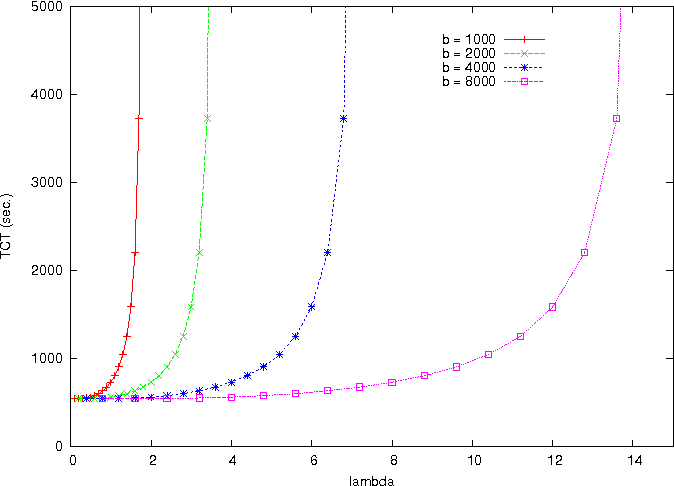
\includegraphics[scale=0.55]{immagini/Fig5-M-GB-1} 
\caption{Tempo medio di conferma delle transazioni (TCT): caso \textit{senza classe}~\cite[fig. 5]{art3:MG^B1}}
\label{im:confronto-classless} 
\end{figure}
\item \textit{classe L e H}: mostrato in fig.~\ref{im:confronto-classLH}; ciascuna classe ha un tasso degli arrivi diverso, rispettivamente $\lambda_L$ e $\lambda_H$. Il grafico mostra il tempo medio in funzione di $\lambda_L$ tenendo costante $\lambda_H$ al valore $\lambda_H=0.2535592656$ (valore calcolato a partire dalle statistiche fornite nel sito Bitcoin). I risultati mostrano quello che ci si aspettava, ovvero il tempo di conferma \`e minore per le transazioni di classe H. Anche in questo caso, aumentare la dimensione dei blocchi non riduce considerevolmente il problema (fig.~\ref{im:confronto-classLH}).
\begin{figure}[!ht]
\centering 
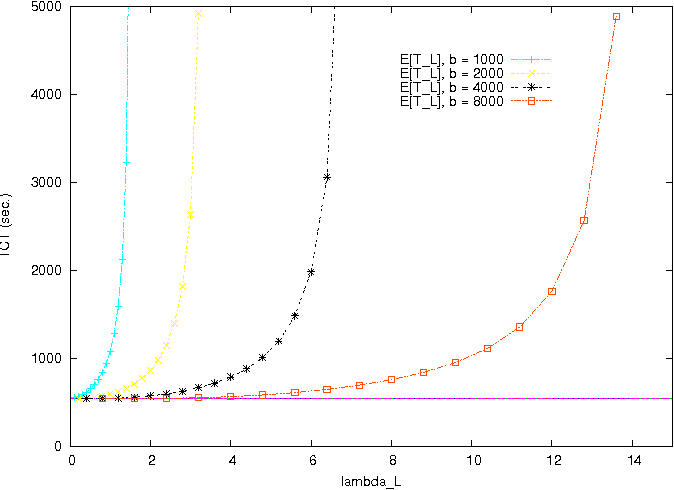
\includegraphics[scale=0.70]{immagini/Fig6-M-GB-1} 
\caption{Tempo medio di conferma delle transazioni (TCT): caso \textit{classe L e H}~\cite[fig. 6]{art3:MG^B1}}
\label{im:confronto-classLH} 
\end{figure}
\end{itemize}

%*****************************************************************
\section{Analisi del modello M/D/1}
Il modello M/D/1 \`e un caso particolare di M/G/1, dove il tempo di servizio \`e costante: $y=T$~\cite{libro:tele}.
La statistica del tempo di servizio $y$ \`e la seguente:
\begin{equation}p_y(a)=\delta(a-T), \quad m_y=T, \quad \sigma_y^2=0. \end{equation}
Gli arrivi rimangono un processo poissoniano con tasso $\lambda$.
Per i calcoli dei momenti delle metriche, si consiglia di vedere~\cite[590]{libro:tele}.\\
La scelta del tempo di servizio \`e un compromesso tra i seguenti criteri:
\begin{itemize}
\item non deve essere troppo grande, perch\`e in tal caso, un utente malintenzionato che ha appena speso le sue criptovalute, potrebbe in quel tempo sfruttarne la vulnerabilità e fare un double-spending; 
\item non essere troppo corto, perch\`e la soluzione del PoW deve essere tale da non poter essere truccata e, se si avesse a disposizione poco tempo, questo rischio potrebbe verificarsi perch\`e verrebbe scelta una soluzione ``banale".
\end{itemize}
